\documentclass[fullscreen=true, bookmarks=true, hyperref={pdfencoding=unicode}]{beamer}
\usepackage[utf8]{inputenc}                                % Кодировка
\usepackage[english,russian]{babel}                        % Переносы
\usepackage{xcolor}                                        % Работа с цветом
\usepackage{amsmath,amssymb,amsfonts}                      % Символы АМО
\usepackage{graphicx}                                      % Графика
\usepackage[labelsep=period]{caption}                      % Разделитель в подписях к рисункам и таблицам
\usepackage{hhline}                                        % Для верстки линий в таблицах
\usepackage{tikz}                                          % Для простых рисунков в документе
\usepackage{fancybox}                                      % Пакет для отрисовки рамок
\usepackage{verbatim}                                      % Для вставки кода в презентацию
\usepackage{animate}                                       % Для вставки видео в презентацию
\usepackage{xmpmulti}                                      % Для вставки gif в презентацию
\usepackage{multirow}
\usepackage{mathrsfs}
\usepackage[normalem]{ulem}

\usetikzlibrary{arrows, snakes, backgrounds}                 % Для отрисовки стрелок
\usetikzlibrary{positioning, fit, arrows.meta, shapes, calc}
% used to avoid putting the same thing several times...
% Command \empt{var1}{var2}
\newcommand{\empt}[2]{$#1^{\langle #2 \rangle}$}

\graphicspath{{images/}}                                   % Путь до рисунков
\setbeamertemplate{caption}[numbered]                      % Включение нумерации рисунков

\definecolor{links}{HTML}{2A1B81}                          % blue for url links
\hypersetup{colorlinks,linkcolor=,urlcolor=links}          % nothing for others

\usetheme{boxes}
\usecolortheme{crane}

\usepackage{pythonhighlight}

\newtheorem*{question}{Вопрос}

\title{Лекция 14. Активное обучение}
\author{Александр Юрьевич Авдюшенко}
\institute{МКН СПбГУ}
\date{19 мая 2022}
\titlegraphic{
\includegraphics[keepaspectratio,width=0.5\textwidth]{logo_fmkn.png}}


\begin{document}
%\unitlength=2mm

% выводим заглавие
\begin{frame}
\transdissolve[duration=0.2]
\titlepage
\end{frame}


\begin{frame}
  \frametitle{Пятиминутка}
  \begin{itemize}
    \item Какую проблему решает аппроксимированный метод кросс-энтропии?
    \item В чем заключаются допущения Маркова?
    \item Расшифруйте аббревиатуру DQN
  \end{itemize}
\end{frame}


\begin{frame}
  \frametitle{Постановка задачи активного обучения}

  Как обычно обучаем модель $a: X \to Y$ по выборке $(x_i, y_i)$, но получение ответов $y_i = y(x_i)$ стоит дорого

  \begin{center}
    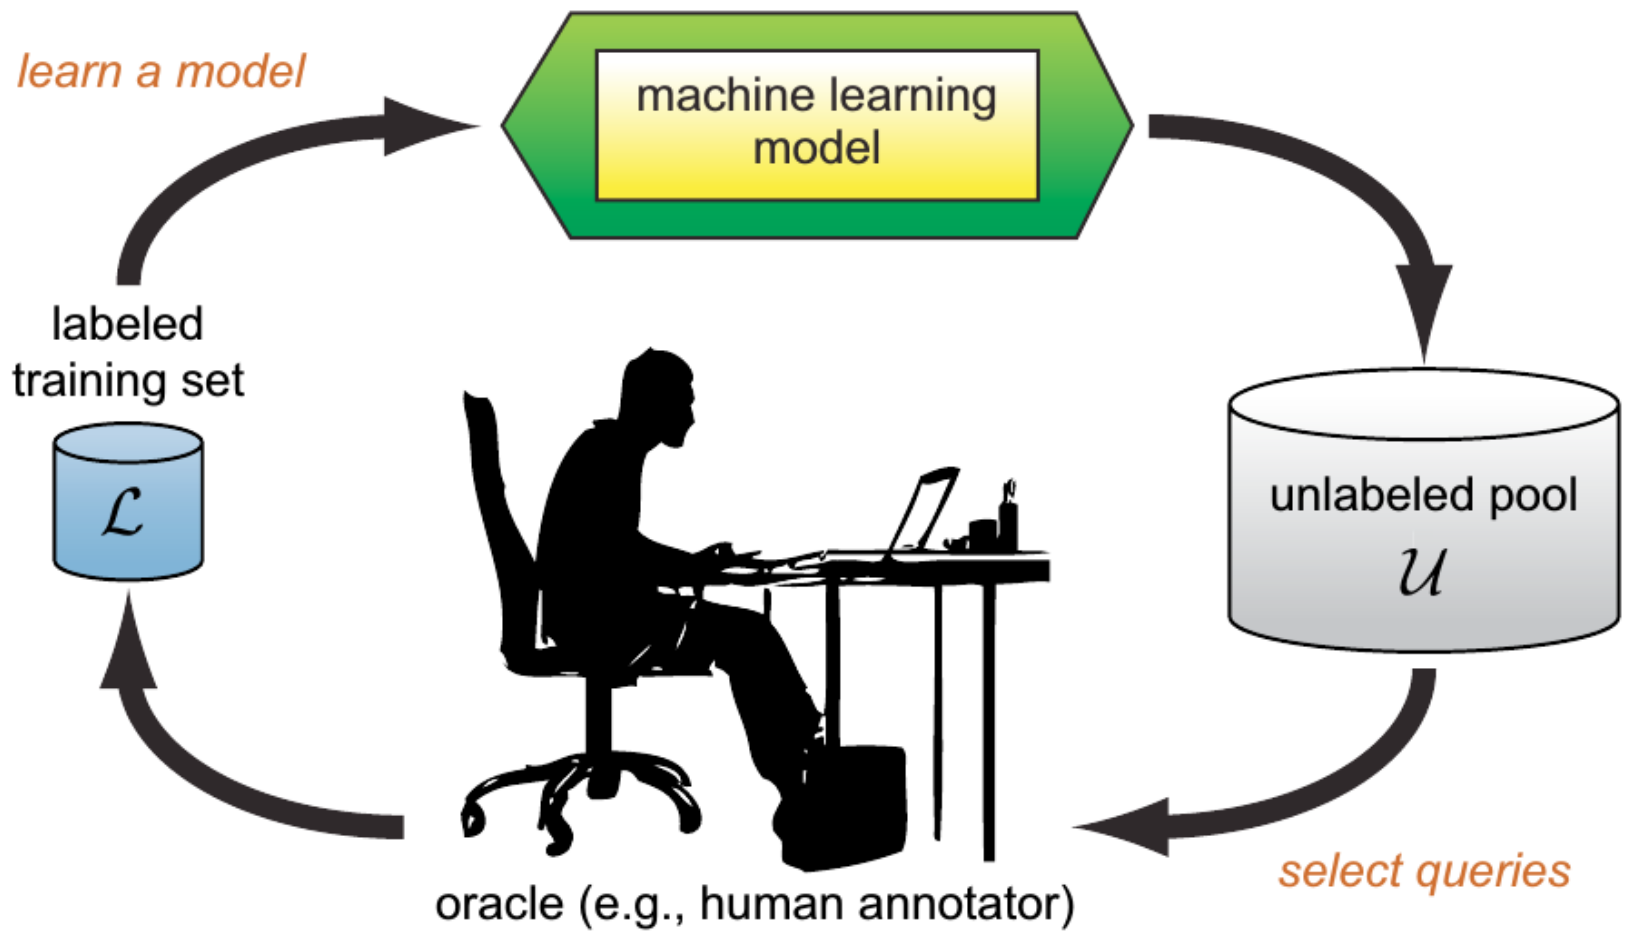
\includegraphics[keepaspectratio,
                     width=.7\paperwidth]{active_learning_scheme.png}
  \end{center}

  \noindent\rule{8cm}{0.4pt}

  {\small
  {\it Burr Settles.} Active Learning Literature Survey. Computer Sciences Tech-
  nical Report 1648, University of Wisconsin–Madison. 2009}
\end{frame}


\begin{frame}
  \frametitle{Постановка задачи активного обучения}

  Как обычно обучаем модель $a: X \to Y$ по выборке $(x_i, y_i)$, но получение ответов $y_i = y(x_i)$ стоит дорого

  \vspace{0.5cm}
  {\bf Вход}: $X^\ell = (x_i, y_i)_{i=1}^\ell$ — выборка размеченных объектов;

    $U = (u_i)_{k=1}^K$ — выборка (пул) неразмеченных объектов

  {\bf Выход}: модель $a$ и размеченная выборка $(u_i, y_i^*)_{i=1}^k, k \leq K$

  \begin{block}{Алгоритм}
    обучить модель по начальной выборке $X^\ell$

    {\bf пока} есть ресурс на разметку и модель не обучилась

    $
    \left[
    \begin{array}{l}
      u_i = \arg\max\limits_{u \in U} \phi(u) \text{ — выбрать неразмеченный объект} \\
      \text{узнать для него } y_i^* = y(u_i) \\
      \text{дообучить модель } a(x) \text{ ещё на одном примере } (u_i, y_i^*)
    \end{array}
    \right.
    $
  \end{block}

  {\bf Цель}: достичь как можно лучшего качества модели $a$, использовав как можно меньше дополнительных примеров $k$
\end{frame}


\begin{frame}
  \frametitle{Почему активное обучение быстрее пассивного?}

  \pause
  {\bf Пример 1}. Синтетические данные: $\ell = 30, \ell + k = 400$

  \begin{itemize}
    \item[(a)] два нормальных распределения
    \item[(b)] логистическая регрессия по 30 случайным объектам
    \item[(c)] логистическая регрессия по 30 отобранным при активном обучении объектам
  \end{itemize}

  \begin{center}
    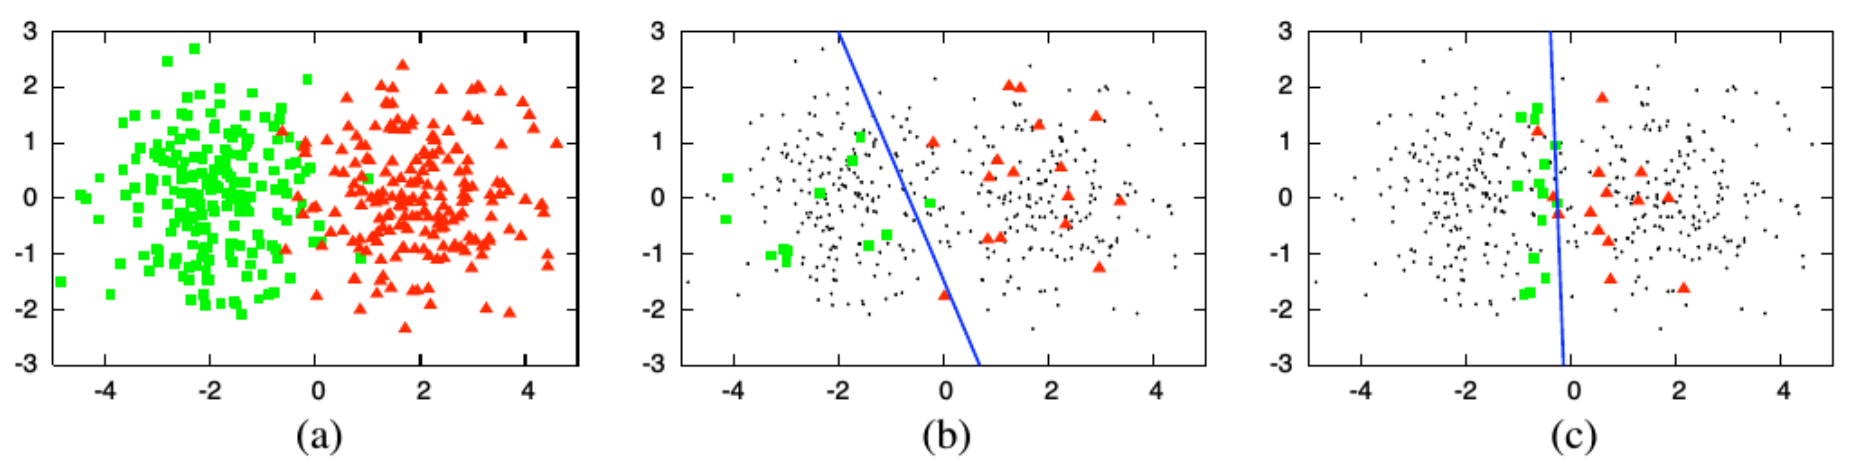
\includegraphics[keepaspectratio,
                     width=.8\paperwidth]{active_learning_LR.png}
  \end{center}

  Обучение по смещённой неслучайной выборке требует меньше данных для построения алгоритма сопоставимого качества.

\end{frame}


\begin{frame}

  {\bf Пример 2}. Одномерная задача с пороговым классификатором.

  $$ x_i \sim \text{uniform}[-1, +1], \quad y_i = [x_i > 0], \quad a(x, \theta) = [x > \theta]$$

  Оценим число шагов для определения $\theta$ с точностью $\frac{1}{k}$:
  \begin{itemize}
    \item Наивная стратегия: выбирать $ u_i \sim \text{uniform}(U)$ — число шагов $O(k)$
    \item Бинарный поиск: выбирать $ u_i $, ближайший к середине зазора между классами $\frac{1}{2} \left( \max\limits_{y_j=0}(x_j) + \min\limits_{y_j=1}(x_j) \right)$ — число шагов $O(log k)$
  \end{itemize}

  \begin{center}
    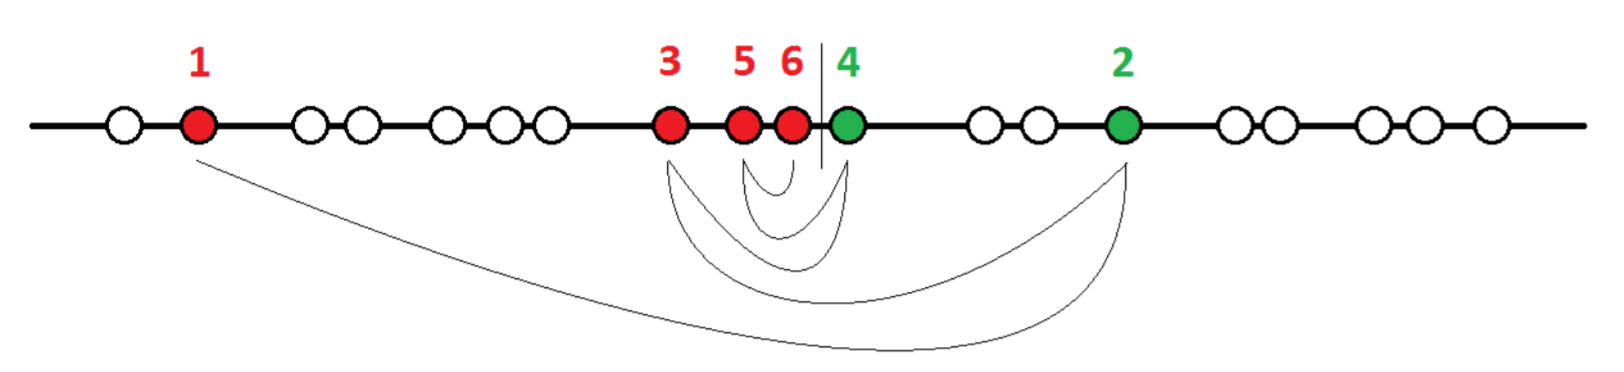
\includegraphics[keepaspectratio,
                     width=.8\paperwidth]{bin_search.png}
  \end{center}

\end{frame}


\begin{frame}
  \frametitle{Оценивание качества активного обучения}
    Кривая обучения (learning curve) — зависимость качества модели на тесте от числа размеченных объектов $k$

  \begin{center}
    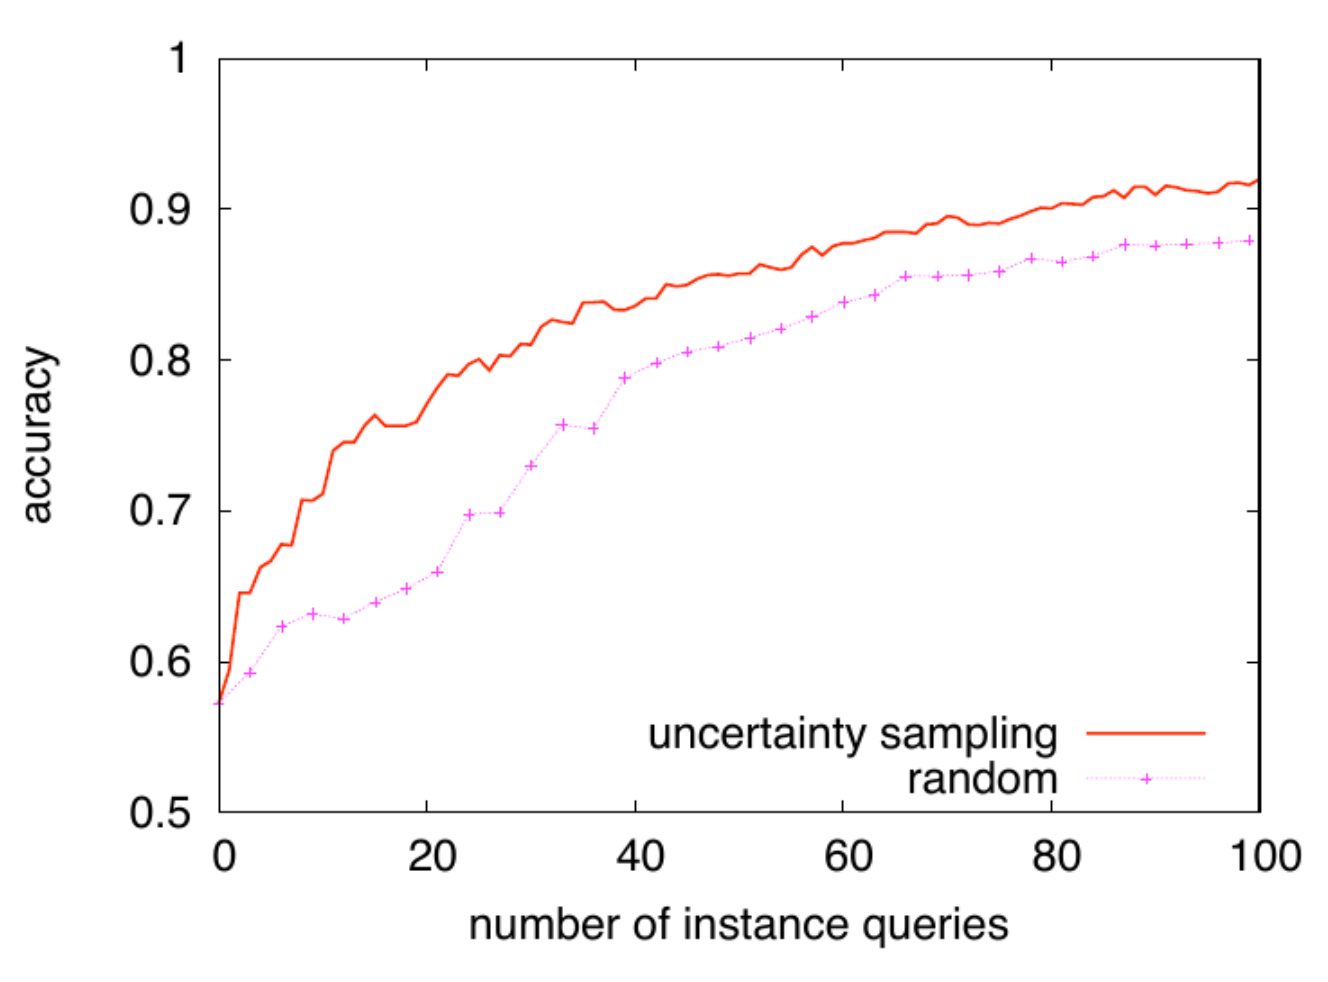
\includegraphics[keepaspectratio,
                     width=.6\paperwidth]{learning_curve.png}

    Бинарная классификация текстов (baseball VS hockey) с помощью логистической регрессии
  \end{center}

\end{frame}


\begin{frame}
  \frametitle{Стратегии активного обучения}

  \begin{itemize}
    \item {\color{brown} Отбор объектов из выборки (pool-based sampling)}:

    какой следующий $u_i$ выбрать из множества $U = \{u_i\}_{i=1}^K$

    \item {\color{brown} Синтез объектов (query synthesis), планирование эксперимента}:

    на каждом шаге синтезировать оптимальный объект $u_i$

    \item {\color{brown} Отбор объектов из потока (selective sampling)}:

    для каждого приходящего $u_i$ решать, стоит ли узнавать $y^*_i$
  \end{itemize}

    Функционал качества модели $a(x,\theta)$ с параметром $\theta$:

    $$ \sum\limits_{i=1}^\ell \mathscr{L}(x_i, y_i; \theta) + \sum\limits_{i=1}^k C_i \mathscr{L}(u_i, y_i^*; \theta) \to \min\limits_{\theta}$$

    где $\mathscr{L}$ — функция потерь, $C_i$ — стоимость информации $y(u_i)$ для методов, чувствительных к стоимости (cost-sensitive)

\end{frame}


\begin{frame}
  \frametitle{Применения активного обучения}

  \begin{itemize}
    \item сбор асессорских данных для информационного поиска и вообще задач машинного обучения
    \item в том числе на платформах краудсорсинга \item планирование экспериментов в естественных науках (пример — комбинаторная химия)
    \item оптимизация трудно вычислимых функций
      (пример — поиск в пространстве гиперпараметров)
  \end{itemize}

  {\bf Применения в бизнесе}:
  \begin{itemize}
    \item управление ценами и ассортиментом в торговых сетях
    \item выбор товара для проведения маркетинговой акции
    \item проактивное взаимодействие с клиентами
    \item выборочный контроль качества
    \item выявление аномалий в данных, случаев мошенничества
  \end{itemize}

\end{frame}


\begin{frame}
  \frametitle{Сэмплирование по неуверенности (uncertainty sampling)}

  {\bf Идея}: выбирать $u_i$ с наибольшей неопределённостью $a(u_i)$

  \begin{block}{Задача многоклассовой классификации}
    \centerline{$ a(u) = \arg\max\limits_{y\in Y} P(y|u) $}

    {\small $p_m(u), m=1\dots |Y|$ — ранжированные по убыванию $P(y|u), y \in Y$}
  \end{block}

  \begin{itemize}
    \item Принцип наименьшей достоверности (lеast сопfidence):
    $$u_i = \arg\min\limits_{u\in U} p_1(u)$$

    \item Принцип наименьшей разности отступов (margin sampling):
    $$u_i = \arg\min\limits_{u\in U} \left( p_1(u) - p_2(u) \right)$$

    \item Принцип максимума энтропии (maximum entropy):
    $$u_i = \arg\min\limits_{x\in U} \sum\limits_{m} p_m(u) \ln p_m(u)$$

  \end{itemize}

\end{frame}

\begin{frame}
  \frametitle{Сэмплирование по неуверенности (uncertainty sampling)}

  В случае двух классов эти три принципа эквивалентны.

  В случае многих классов появляются различия.

  \vspace{0.5cm}
  {\bf Пример}. Три класса, $p_1 + p_2 + p_3 = 1$

  Показаны линии уровни трёх критериев выбора объекта:

  \begin{center}
    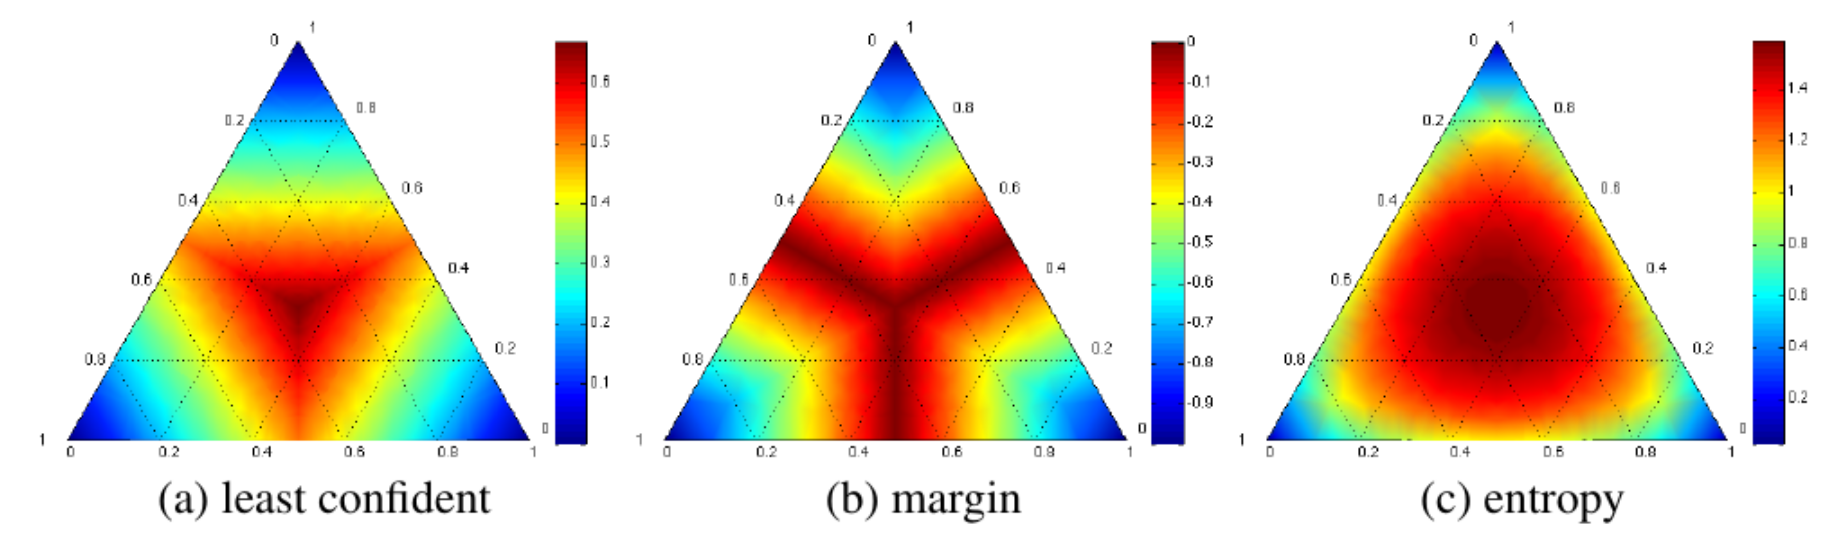
\includegraphics[keepaspectratio,
                     width=.9\paperwidth]{three_uncertaincy_principles.png}
  \end{center}

  \noindent\rule{8cm}{0.4pt}

  {\small
  {\it Burr Settles.} Active Learning Literature Survey. Computer Sciences Tech-
  nical Report 1648, University of Wisconsin–Madison. 2009}

\end{frame}


\begin{frame}
  \frametitle{По несогласию в комитете (query by committee)}

  {\bf Идея}: выбирать $u_i$ с наибольшей несогласованностью решений
  комитета моделей $a_t(u_i) = \arg\max\limits_{y \in Y} P_t(y|u_i), t=1, \dots, T$

  \begin{itemize}
    \item Принцип {\it максимума энтропии} —
      выбираем $u_i$, на котором $a_t(u_i)$ максимально различны:
      $$ u_i = \arg\min\limits_{u \in U} \sum\limits_{y\in Y} \hat p(y|u) \ln \hat p(y|u), $$
      где $\hat p(y|u) = \frac{1}{T} \sum\limits_{t=1}^T \left[a_t(u) = y \right]$
    \item Принцип максимума средней {\it KL-дивергенции} —
      выбираем $u_i$, на котором $P_t(y|u_i)$ максимально различны:
      $$ u_i = \arg\max\limits_{u \in U} \sum\limits_{t=1}^T KL \left(P_t (y|u) \| \overline P (y|u)\right), $$
      где $\overline P (y|u) = \frac{1}{T} \sum\limits_{t=1}^T P_t(y|u)$ — консенсус комитета
  \end{itemize}

\end{frame}


\begin{frame}
  \frametitle{Сокращение пространства решений (version space reduction)}

  {\bf Идея}: выбирать $u_i$, максимально сужая множество решений.

  {\bf Пример}. Пространства допустимых решений для линейных и пороговых классификаторов (двумерный случай):

  \begin{center}
    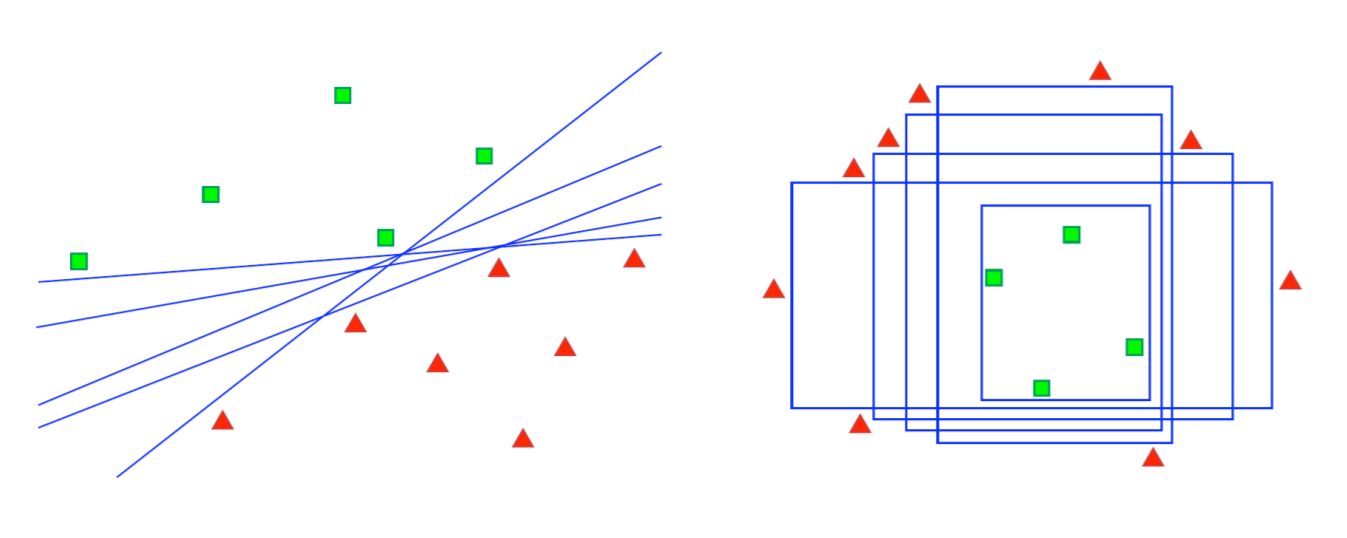
\includegraphics[keepaspectratio,
                     width=.7\paperwidth]{solution_space.png}
  \end{center}

  Бустинг и бэггинг находят конечные подмножества решений.

  Поэтому сэмплирование по несогласию в комитете — это аппроксимация принципа сокращения пространства решений.

\end{frame}


\begin{frame}
  \frametitle{Ожидаемое изменение модели (ехресted model change)}

  {\bf Идея}: выбрать $u_i$, который в методе стохастического градиента привёл бы к наибольшему изменению модели.

  Параметрическая модель многоклассовой классификации:

  $$ a(u, \theta) = \arg\max\limits_{y \in Y} P(y|u, \theta)$$

  Для каждого $u \in U$ и $y \in Y$ оценим длину градиентного шага в пространстве параметров $\theta$ при дообучении модели на $(u,y)$;
  пусть $\nabla_\theta \mathscr{L}(u,y; \theta)$ — вектор градиента функции потерь.

  \vspace{0.5cm}
  Принцип максимума {\it ожидаемой длины градиента}:

 $$ u_i = \arg\max\limits_{u \in U} \sum\limits_{y \in Y} P(y| u, \theta) \| \nabla_\theta \mathscr{L}(u,y; \theta) \| $$
\end{frame}


\begin{frame}
  \frametitle{Ожидаемое сокращение ошибки (expected error reduction)}

  {\bf Идея}: выбирать $u_i$, который после дообучения даст наиболее
  уверенную классификацию неразмеченной выборки $U \backslash u_i$.

  Для каждого $u \in U$ и $y \in Y$ обучим модель классификации,
  добавив к размеченной обучающей выборке $X^\ell$ пример $(u,y)$:

  $$ a_{uy}(x) = \arg\max\limits_{z \in Y} P_{uy}(z|x)$$

  \begin{itemize}
    \item Принцип максимума {\it уверенности на неразмеченных данных}:
    $$ u_i = \arg\max\limits_{u \in U} \sum\limits_{y \in Y} P(y|u) \sum\limits_{u_j \in U \backslash u }
    P_{uy}(a_{uy}(u_j) | u_j)$$
    \item Принцип минимума {\it энтропии неразмеченных данных}:
    $$ u_i = \arg\max\limits_{u \in U} \sum\limits_{y \in Y} P(y|u) \sum\limits_{u_j \in U \backslash u }
    \sum\limits_{z \in Y} P_{uy}(z|u_j) \log P_{uy} (z | u_j)$$
  \end{itemize}

\end{frame}


\begin{frame}
  \frametitle{Безградиентная оптимизация. Метод Нелдера—Мида}

  {\bf Идея}: выбирать объекты $u_i$ не из конечного пула, а из всего $X$, максимизируя $\max\limits_{u \in X} \phi(u)$ любым безградиентным методом.

  {\bf Метод Нелдера—Мида}: перемещение и деформирование симплекса из $n+1$ точек в пространстве $X$ размерности $n$

  \begin{center}
    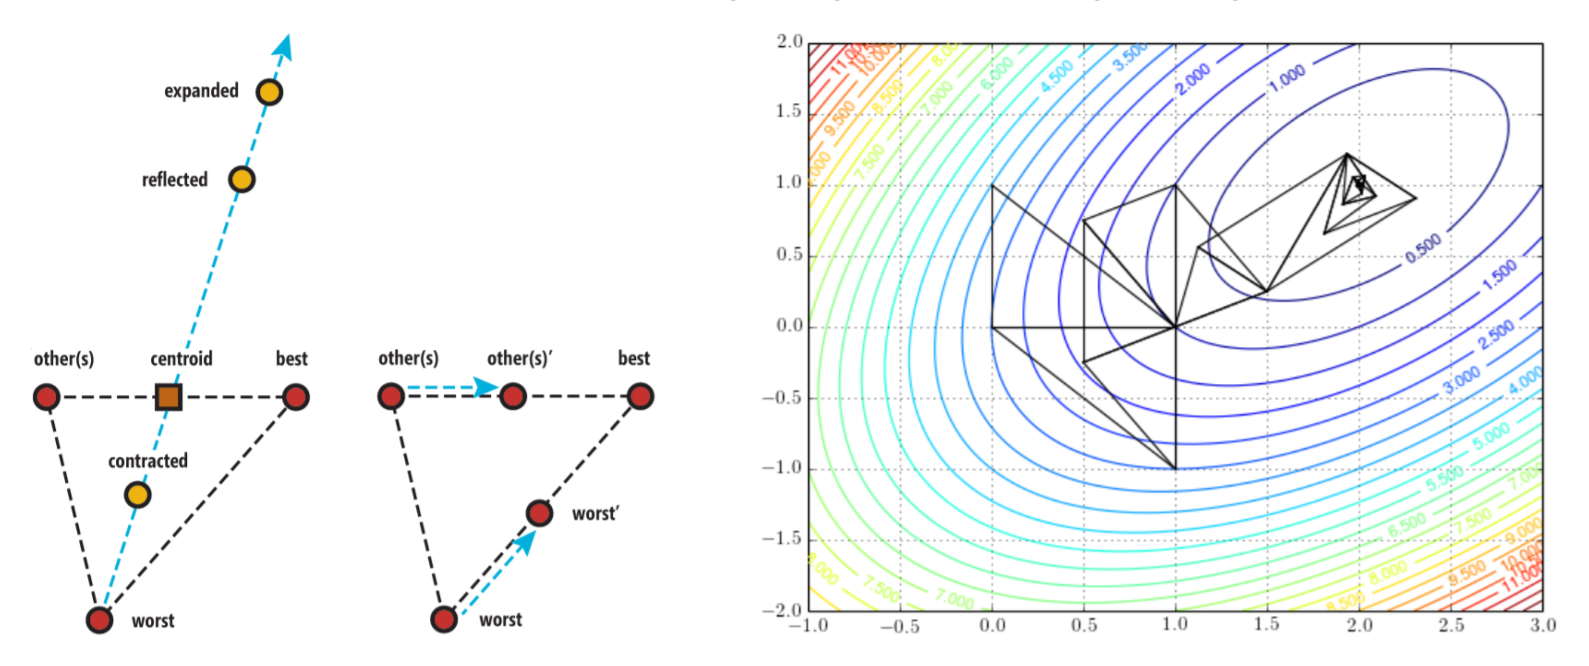
\includegraphics[keepaspectratio,
                     width=.85\paperwidth]{nelder_mead.png}
  \end{center}

  \noindent\rule{8cm}{0.4pt}

  {\small
  {\it J.A.Nelder, R.Mead}. A simplex method for function minimization. 1965.}

\end{frame}


\begin{frame}
  \frametitle{Сокращение дисперсии (variance reduction)}

  {\bf Идея}: выбирать $u \in X$, который даст наименьшую оценку дисперсии $\sigma_a^2(u)$ после дообучения модели $a(x, \theta)$.

  Задача регрессии, метод наименьших квадратов:
  $$ S^2(\theta) = \frac{1}{\ell} \sum\limits_{i=1}^\ell \left(a(x_i, \theta)-y_i \right)^2 \to \min\limits_{\theta} $$

  Из теории {\it оптимального планирования экспериментов} (OED, optimal experiment design):
  $$ u = \arg\max\limits_{u \in U} \sigma^2_a(u),\quad \sigma^2_a(u) \approx S^2
  \left( \frac{\partial a(u)}{\partial \theta} \right)^T
  \left( \frac{\partial S^2}{\partial \theta^2} \right)^{-1}
  \left( \frac{\partial a(u)}{\partial \theta} \right)
  $$

  В частности, для линейной регрессии
  $$ \sigma_a^2(u) \approx S^2 u^T (F^T F)^{-1} u, $$

  где $F$ — матрица объекты-признаки

\end{frame}


\begin{frame}
  \frametitle{Взвешивание по плотности (density-weighted methods)}

  {\bf Идея}: понижать вес нерепрезентативных  объектов

  \begin{columns}
    \begin{column}{.4\paperwidth}
      {\bf Пример}. Объект $A$ более пограничный, но менее  репрезентативный, чем $B$
    \end{column}
    \begin{column}{.4\paperwidth}
      \begin{center}
        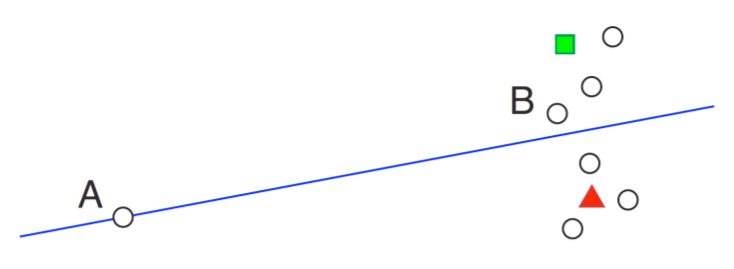
\includegraphics[keepaspectratio,
                         width=.4\paperwidth]{density_weighted.png}
      \end{center}
    \end{column}
  \end{columns}


  Любой критерий выбора объектов, имеющий вид
  $$ u = \arg\max\limits_{u \in U} \phi(u) $$

  может быть уточнён локальной оценкой плотности:
  $$ u = \arg\max\limits_{u \in U} \phi(u) \left(
  \sum\limits_{u^\prime \in U} \text{sim}(u,u^\prime) \right)^\beta,$$
  $\text{sim}(u,u^\prime)$ — оценка близости $u$ и $u^\prime$ (чем ближе, тем больше)

\end{frame}


\begin{frame}
  \frametitle{Необходимость изучающих действий в активном обучении}

  {\bf Недостатки} стратегий активного обучения:
  \begin{itemize}
    \item остаются не обследованные области пространства $X$
    \item в результате снижается качество обучения
    \item увеличивается время обучения
  \end{itemize}

  \vspace{0.5cm}
  {\bf Идеи} применения изучающих действий:
  \begin{itemize}
    \item брать случайный объект с вероятностью $\varepsilon$
    \item адаптировать параметр $\varepsilon$ в зависимости от успешности изучающих действий
    \item использовать обучение с подкреплением
  \end{itemize}

  \noindent\rule{8cm}{0.4pt}

  {\small
  {\it Djallel Bouneffouf}. Exponentiated gradient exploration for active learning. 2016.

  {\it Djallel Bouneffouf}. Contextual bandit for active learning: active Thompson sampling. 2014.
  }

\end{frame}


\begin{frame}
  \begin{question}
    Придумайте обёртку $\varepsilon$-active для любого алгоритма активного обучения
  \end{question}

  \vspace{1cm}
  \pause
  {\bf Проблемы}:
  \begin{itemize}
    \item как подбирать вероятность $\varepsilon$ исследовательских действий?
    \item как её адаптировать (уменьшать) со временем?
  \end{itemize}

\end{frame}


\begin{frame}
  \frametitle{Экспоненциальный градиент (exponential gradient)}

  $\varepsilon_1, \dots, \varepsilon_H$ — сетка значений параметра $\varepsilon$

  $p_1,\dots,p_H$ — вероятности использовать значения $\varepsilon_1, \dots, \varepsilon_H$

  $\beta, \tau, \kappa$ — параметры метода

  {\bf Идея} алгоритма ЕG-active: аналогично алгоритму AdaBoost, экспоненциально увеличивать $p_h$ в случае успеха $\varepsilon_H$

  \begin{itemize}
    \item экспоненциальное обновление весов $w_h$ по значению критерия $\phi(u_i)$ на выбранном объекте $u_i$:
    $$ w_h := w_h \exp \left(\frac{\tau}{p_h}(\phi(u_i) + \beta) \right) $$
    \item перенормировка вероятностей:
    $$ p_h := (1-\kappa) \frac{w_h}{\sum_j w_j} + \kappa \frac{1}{H} $$
  \end{itemize}

  \noindent\rule{8cm}{0.4pt}

  {\small
  {\it Djallel Bouneffouf}. Exponentiated gradient exploration for active learning. 2016.}

\end{frame}


\begin{frame}
  \frametitle{Активное обучение, когда аннотаторов много}

  $y_{it}$ — ответы аннотаторов $t \in T$ на объекте $u_i$

  {\bf Задача}: сформировать согласованный «правильный» ответ $\hat y_i$

  и оценить надёжность каждого аннотатора $q_t = P[y_{it} = \hat y_i]$

  \begin{center}
    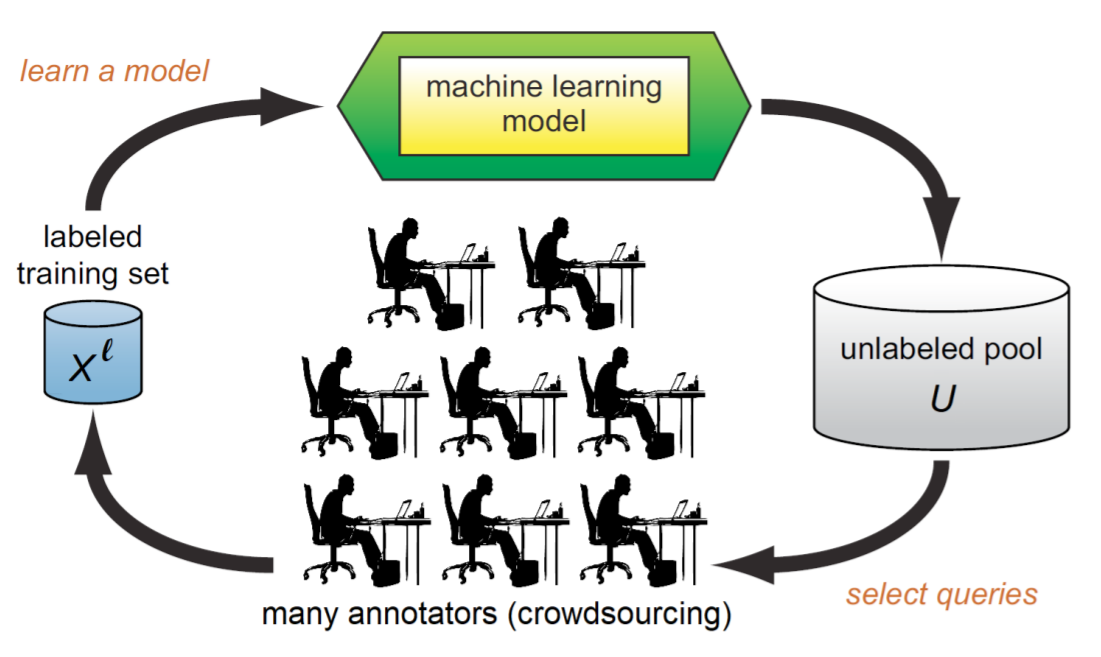
\includegraphics[keepaspectratio,
                     width=.65\paperwidth]{AL_crowd.png}
  \end{center}

  \noindent\rule{8cm}{0.4pt}

  {\small
  {\it Р.А.Гилязев‚ Д.Ю.Турдаков}. Активное обучение и краудсорсинг: обзор
  методов оптимизации разметки данных. 2018.}

\end{frame}


\begin{frame}
  \frametitle{Согласование оценок аннотаторов}

  $y_{it}$ — ответы аннотаторов $t \in T$ на объекте $u_i$

  $T_i \subset T$ — множество аннотаторов, разметивших объект $u_i$

  \begin{block}{Взвешенное голосование аннотаторов}
    $$ \hat y_i = \arg \max\limits_{y\in Y}
    \sum\limits_{t \in T_i} w_t [y_{it} = y]$$

    $w_t$ — вес аннотатора при голосовании

    $w_t = 1$ при голосовании по большинству (majority voting)

    $w_t = \log \frac{q_t}{1-q_t}$ при предположении, что аннотаторы независимы
  \end{block}

  {\bf ЕМ-подобный алгоритм} согласования аннотаций объекта $u_i$:

  {\color{brown} пока} оценки не сойдутся
  \begin{itemize}
    \item оценить правильный ответ $\hat y_i$
    \item оценить надёжности $q_t$ и веса $w_t$ аннотаторов
    \item если $q_t < \delta$ то исключить аннотатора из оценки
  \end{itemize}

\end{frame}


\begin{frame}
  \frametitle{Варианты моделирования надёжности аннотаторов}

  \begin{itemize}
    \item По результатам выполнения тестовых заданий (ханипоты, honeypots)
    \item Моделирование матрицы ошибок $|Y|\times|Y|$:
    $$ \pi_{yz}^t = P[\text{аннотатор } t \text{ ставит } z \text{ вместо }y], \quad y, z \in Y$$
    \item Моделирование трудности объектов:
    $$ q_t(u_i) = \sigma \left(\frac{\alpha_t}{\beta_i} \right) = \frac{1}{1 + \exp\left(-\frac{\alpha_t}{\beta_i} \right) },$$
    $\alpha_t$ — частотная оценка надёжности аннотатора $t$
    $\beta_i$ — оценка трудности объекта $u_i$ (по большому $|T_i|$)
    \item Моделирование тематической компетентности аннотаторов:
      $p(\text{topic}|u_i)$ — тематическое векторное представление
      объекта $u_i$, например, если объект является текстом
  \end{itemize}

\end{frame}


\begin{frame}
  \frametitle{Задача назначения заданий аннотаторам}

  Общая схема распределения заданий:
  $$\begin{cases}
    u_i = \arg\max\limits_{u \in U} \phi (u) \text{ — выбор неразмеченного объекта в AL} \\
    t = \arg\max\limits_{t \in T} q_t (u_i) \text{ — выбор наиболее уверенного аннотатора}
  \end{cases}$$
  Обучение вероятностной модели уверенности аннотатора
  $q_t(u_i, \theta_t) = \sigma(\theta_t^Tu_i)$ на размеченных им объектах $U_t$:
  $$ \sum\limits_{u_i \in U_t} (y_{it} = \hat y_{i}) q_t(u_i, \theta_t) +
  (y_{it} \neq \hat y_{i})(1 - q_t(u_i, \theta_t)) \to \max\limits_{\theta_t} $$

  {\bf Недостаток}: одни аннотаторы будут выбираться слишком
  часто, другие не будут выбираться совсем

  {\bf Сэмплирование аннотаторов}: $t \sim q_t(u_i)p(t)$ с учётом
  априорной информации $p(t)$ о средней надёжности $q_t$, опыте,
  текущей доступности, объёме проделанной работы

\end{frame}

\begin{frame}[t]
  \frametitle{Резюме}

  \begin{itemize}
    \item Активное обучение используется для уменьшения
    обучающей выборки, когда размеченные данные дороги
    \item При малом объёме размеченных данных оно достигает
    того же качества, что пассивное при полной разметке
    \item Два основных типа активного обучения:
    выбор объектов из пула и синтез новых объектов
    \item Введение изучающих действий в активном обучении
    позволяет ещё быстрее обследовать пространство $X$
    \item В краудсорсинге активное обучение совмещается
    с оцениванием надёжности аннотаторов и трудности
    заданий при распределении заданий по аннотаторам
  \end{itemize}

  \vspace{0.25cm}
  \pause
  Что ещё можно посмотреть?

  \begin{itemize}
    \item Краудсорсинг в Яндекс.Толоке: \href{https://toloka.ai}{https://toloka.ai}
    \item Pengzhen Ren et al. A survey of deep active learning. 2020
  \end{itemize}
\end{frame}

\end{document}
